Trabaje para $t\ge0$ con la transformada unilateral de Laplace y entradas causales. Use $H(t-a)=0$ para $t<a$ y $H(t-a)=1$ para $t\ge a$; los valores aislados en saltos no alteran la transformada. Sea
\[f(t)=\begin{cases}9-t^2,&0\le t<3,\\0,&t\ge3.\end{cases}\]
La gráfica de $g$ es una versión de esta parábola con las escalas indicadas, y es cero después del arco.
\begin{center}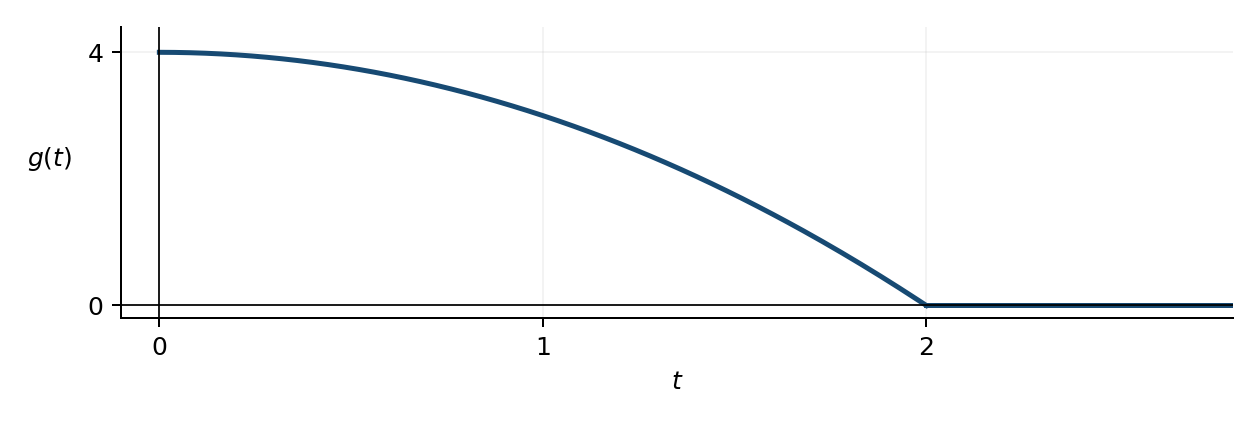
\includegraphics[width=.9\linewidth]{assets/M2-E0228-input.png}\end{center}

\begin{enumerate}[label=(\alph*),ref=\alph*,leftmargin=*]
\item Calcule la transformada de $f$.
\item Utilizando el resultado anterior, calcule la transformada de $g$.
\item Resuelva $y''+y=f(t)$, $y(0)=y'(0)=0$.
\end{enumerate}
